\subsection{Recurrent Neural Networks} 
Mô hình RNN (Recurrent Neural Network) giữ một trạng thái ẩn (hidden state) và sử dụng nó để lưu trữ thông tin từ các bước thời gian trước đó. Điều này cho phép RNN hiểu và xử lý các dữ liệu dạng chuỗi, chẳng hạn như văn bản, âm thanh hoặc dữ liệu thời gian.
\begin{figure}[h]
    \centering
    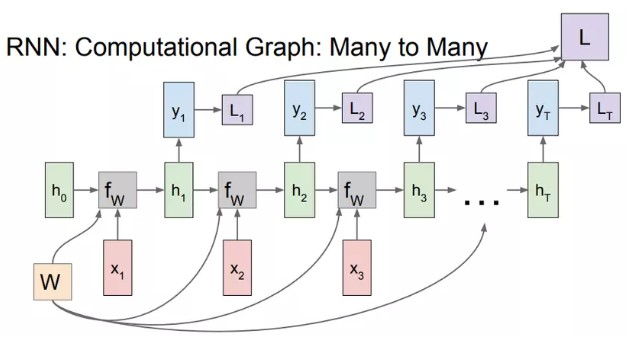
\includegraphics[width=0.5\textwidth]{bibliography/pictures/RNN.jpg}
    \caption{Mô hình Many to Many}
\end{figure}

\begin{itemize}  
    \item \textbf{Mô hình Many to Many của RNN:}
    \begin{itemize}
        \item Mạng Neural Network thông thường bao gồm các lớp: lớp đầu vào (input layer) \( x \), lớp ẩn (hidden layer) \( h \), và lớp đầu ra (output layer) \( y \). Tất cả các lớp này được kết nối đầy đủ với nhau.
        \item Trong RNN, đầu vào tại mỗi thời điểm \( x_t \) sẽ được kết hợp với lớp ẩn từ bước thời gian trước đó \( h_{t-1} \) thông qua hàm \( f_W \) để tính toán ra lớp ẩn hiện tại \( h_t \). Đầu ra tại mỗi thời điểm \( y_t \) sẽ được tính từ lớp ẩn hiện tại \( h_t \), W là tập các trọng số và nó được xuất hiện ở tất cả các cụm, các \( L_1, L_2, \ldots, L_T \) là các hàm mất mát.
        \item Kết quả của các quá trình tính toán trước đã được "nhớ" bằng cách kết hợp thêm \( h_{t-1} \) để tính toán \( h_t \). Điều này giúp tăng độ chính xác cho những dự đoán ở hiện tại.
        \item Hàm \( f_W \) kết hợp \( h_{t-1} \) và \( x_t \) để tính \( h_t \):
        \[
        h_t = f_W(h_{t-1}, x_t)
        \]
        \item Hàm \( f_W \) được định nghĩa cụ thể là hàm \( \tanh \), công thức trên sẽ trở thành:
        \[
        h_t = \tanh(W_{hh}h_{t-1} + W_{xh}x_t)
        \]
        \item Đầu ra \( y_t \) được tính từ \( h_t \):
        \[
        y_t = W_{hy}h_t
        \]
        \item RNN sử dụng 3 ma trận trọng số là \( W_{hh} \) kết hợp với "bộ nhớ trước" \( h_{t-1} \) và \( W_{xh} \) kết hợp với đầu vào hiện tại \( x_t \) để tính toán "bộ nhớ của bước hiện tại" \( h_t \) từ đó kết hợp với \( W_{hy} \) để tính toán đầu ra \( y_t \).
    \end{itemize}
            
    \item \textbf{Các Dạng Mô Hình RNN Khác:}
    \begin{itemize}
        \item Ngoài mô hình Many to Many, RNN còn có các dạng khác như One to One, One to Many, Many to One.
    \end{itemize}
\end{itemize}